\documentclass[%
aip,
amsmath,amssymb,
preprint,%
%reprint,%
%author-year,%
%author-numerical,%
jcp,
showkeys,
]{revtex4-2}

\usepackage{hyperref}

\usepackage{siunitx}
\DeclareSIUnit\rydberg{Ry}
\usepackage{tikz}
\usepackage{paralist}
\usepackage[version=4]{mhchem}
\usepackage{rotating}
\usepackage{chngcntr}

\def\dbe{\ensuremath{\Delta\text{BE}}}

%% Apr 2021: AIP requests that the corresponding 
%% email to be moved after the affiliations
\makeatletter
\def\@email#1#2{%
	\endgroup
	\patchcmd{\titleblock@produce}
	{\frontmatter@RRAPformat}
	{\frontmatter@RRAPformat{\produce@RRAP{*#1\href{mailto:#2}{#2}}}\frontmatter@RRAPformat}
	{}{}
}%
\makeatother

\begin{document}
	
\title{Prediction of XPS binding energies for molecules grafted on calcium surfaces}

\author{Pierre Beaujean}
\email{pierre.beaujean@unamur.be}
\affiliation
{University of Namur, Theoretical Chemistry Lab, Unit of Theoretical and Structural Physical Chemistry, Namur Institute of Structured Matter, rue de Bruxelles, 61, B-5000 Namur (Belgium)}


\author{Benoît Champagne}
\affiliation
{University of Namur, Theoretical Chemistry Lab, Unit of Theoretical and Structural Physical Chemistry, Namur Institute of Structured Matter, rue de Bruxelles, 61, B-5000 Namur (Belgium)}

\date{\today}

\begin{abstract} %% note: 250 words max
	This study investigates the adsorption of tetrahydrofuran (THF) and of its potential degradation products on various calcium surfaces using periodic boundary conditions density functionnal theory calculations. Slabs of metallic calcium (\ce{Ca^0}), calcium oxide (\ce{CaO}), and calcium hydride (\ce{CaH2}) have been modeled, with additional consideration given to full hydroxide coverage on \ce{CaO}. Two primary reaction types were identified: reactions between the carbon atoms of the adsorbates and the surface, particularly with \ce{CO2}, and proton transfer from the alcohol moiety of the adsorbates to the \ce{CaO} surface. To complement the structural insights, simulated X-ray photoelectron spectroscopy (XPS) spectra have been analyzed to provide detailed information on the signatures of the effects of the changes of chemical environment of atoms upon adsorption. 
	So, after a detailed investigation of several methodologies, the Slater-Janak scheme with $E_{ref}=E_\infty$ has been applied to the different systems, showing significant changes in the O 1s and C 1s spectra upon adsorption, while the Ca 2s binding energies are less affected. The signature of the interactions between the oxygen and metallic calcium (\ce{Ca^0}) atoms were also clearly observed in the spectra. Our results align with experimental data, when available.	These findings provide valuable trends for analyzing XPS spectra in the context of solid-electrolyte interphase formation. 
\end{abstract}

\keywords{X-ray photoelectron spectrocopy; surface; adsorption; density functional theory}

\maketitle


\clearpage
\section{Introduction}

Batteries represent a crucial technology for the transition to a climate-neutral society. Since their market introduction, lithium-ion batteries (LIBs) have evolved into a highly mature technology, currently utilized in a wide range of applications.\cite{zubiLithiumionBatteryState2018,kimLithiumionBatteriesOutlook2019} Despite their established performance, LIBs face significant limitations that hinder their suitability for large-scale applications, primarily due to different fundamental issues, one of them being the insufficient energy density.\cite{luReviewKeyIssues2013,li30YearsLithiumIon2018} Addressing this point can be achieved through the use of divalent cations, such as \ce{Ca^2+}.\cite{arroyo-dedompabloAchievementsChallengesProspects2020,taghavi-kahaghPoweringFutureComprehensive2024} However, its high reactivity demands the design of specialized electrolytes to support a reversible mechanism. Additionally, detailed insight into the chemistry of the solid-electrolyte interphase (SEI) remains crucial.\cite{melemedImpactDifferentialCa22023,zhaoRevealingSolidElectrolyte2022}
In the literature, calcium-ion batteries (CIBs) utilize electrolytes such as dimethyl ether (DME), ethylene carbonate (EC), glyme, or tetrahydrofuran (THF), often in combination with weakly coordinating anions like \ce{BH4-} or \ce{BF4-} \cite{songElectrolyteOptimizationInterphase2022,zhaoRevealingSolidElectrolyte2022,bodinBoronBasedFunctionalAdditives2023}. 
Both experimental \cite{songElectrolyteOptimizationInterphase2022,melemedImpactDifferentialCa22023,bodinBoronBasedFunctionalAdditives2023} and quantum chemistry studies \cite{hahnCriticalRoleConfigurational2020,liepinyaComputationalComparisonEther2021,yamijalaStabilityCalciumIon2021} have explored SEI formation, typically focusing on the degradation pathways arising from the interactions between calcium, the electrolyte, and coordinating anions\cite{wuUnderstandingSolidElectrolyte2021,bodinBoronBasedFunctionalAdditives2023}. While these studies provide valuable insights, the comparison between experimental spectroscopic data and simulated spectra is an important aspect that can significantly enhance the understanding, both at the experimental and theoretical level, but it is not always considered.


X-ray photoelectron spectroscopy (XPS) is a surface-sensitive, quantitative spectroscopy that allows for the identification of elements of molecules in different environments. It belongs to the family of photoemission spectroscopies, where the kinetic energy of electrons emitted by the photoelectric effect is analyzed. Specifically, XPS uses a beam of soft X-rays ($\SI{100}{\electronvolt} < h\nu < \SI{10}{\kilo\electronvolt}$), enabling the probing of core electrons (low principal quantum number).\cite{stevieIntroductionXrayPhotoelectron2020} The conservation of energy is described by the equation:
\begin{equation}
	h\nu = \text{BE} + E_{\text{kin}} + \phi, \label{eq:xps}
\end{equation}
where BE is the binding energy of the electron, $E_{\text{kin}}$ is the kinetic energy of the emitted electron (measured by the detector), and $\phi$ is the work function, which accounts for surface effects and detector contributions. Using a source of monochromatic X-rays (such as Al $K_\alpha$, $h\nu = \SI{1486.7}{\electronvolt}$), it is possible to determine BE from $E_{\text{kin}}$ \cite{stevieIntroductionXrayPhotoelectron2020}. The binding energy depends on how tightly the electron is bound in its orbital, making it sensitive to the oxidation state and to the chemical environment of the originating atom. It is routinely used experimentally to gain understanding on the SEI composition of both LIBs and CIBs \cite{forero-saboyaUnderstandingNaturePassivation2020a,songElectrolyteOptimizationInterphase2022,bodinBoronBasedFunctionalAdditives2023,melemedImpactDifferentialCa22023,linDecipheringDynamicInterfacial2024}. However, to the BE'st of our knowledge, while there have been some theoretical studies for the SEI of LIBs via the simulation of the XPS spectra\cite{ebadiInsightsLiMetalOrganic2019}, none exists for CIBs.

Therefore, this study explores the XPS spectra related to the degradation and polymerization of THF, using it as a model system. Several potential degradation products (Fig.~\ref{fig:THFdegradation}), along with the polymerization into poly(tetramethylene ether) glycol (PTMEG), are investigated on various calcium substrates, including calcium oxide and calcium hydride. These molecules are chosen in order to consider different relevant chemical moieties. Following a review of the theoretical methods and the computational details in sections \ref{sec:theo} and \ref{sec:comp}, the results are presented. First, the different protocols for calculating binding energies are evaluated in section \ref{sec:proto}. Then, the geometries of the adsorbed molecules along with their adsorption energies are scrutinized in section \ref{sec:geom}. Finally, the core of the paper is the analysis of the simulated XPS spectra, in section \ref{sec:BE's}.


\begin{figure}[!h]
	\centering
	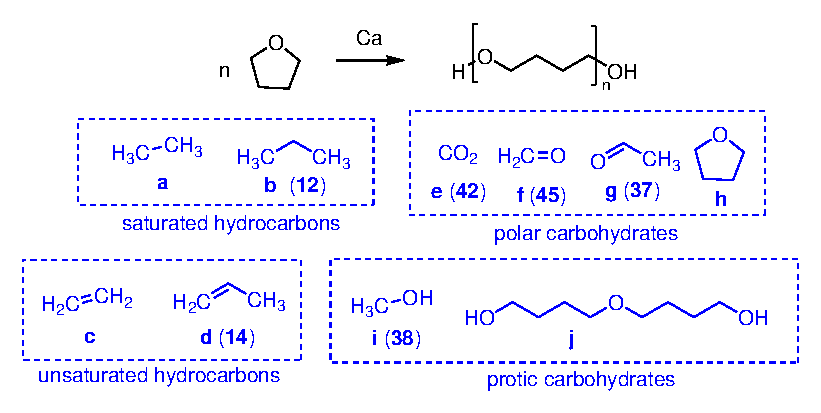
\includegraphics[width=\linewidth]{Figure1}
	\caption{The main polymerization pathway of THF leads to PTMEG (black). \textbf{j} is used as a model for the PTMEG (with n=2), while fragmentation can lead to (un)saturated hydrocarbons (\textbf{a}-\textbf{d}) or oxygen-containing molecules (\textbf{e}-\textbf{i}). Numbers indicate the correspondence with the XPS dataset of Pueyo Bellafont \emph{et al.}\cite{pueyobellafontPerformanceTPSSFunctional2016} (Fig. S1).}
	\label{fig:THFdegradation}
\end{figure}

\section{Theoretical methods}\label{sec:theo}

From a quantum chemistry perspective, the binding energy (here for core electrons) is akin to the ionization energy:
\begin{equation}
	\text{BE}_i = E^{N-1}_i(\text{final}) - E^{N}(\text{initial}), \label{eq:dscf}
\end{equation}
where $E^{N}$ and $E^{N-1}_i$ are the energies of the initial $N$-electron non-ionized state and the final $N-1$ electron ionized state with a electron hole on atom $i$. While these energies could be obtained through (relativistic) multi-configuration approaches, this is impractical for large systems. Even CIS or TD-DFT based calculations of excitation energies are challenging, as they correspond to highly excited states \cite{vinesPredictionCoreLevel2018}.

For gas-phase molecules, classical quantum chemistry tools can be utilized. At the HF level, BE's can be approximated using Koopmans' theorem, which correlates BE's to the orbital energy of the removed electron. This is known as the initial state (IS) or frozen orbitals (FO) approach.\cite{pueyobellafontPredictionCoreLevel2015} However, electronic relaxation effects are neglected. More accurate values can be obtained using Eq.~\eqref{eq:dscf}, by computing the energy difference between initial and final states at the HF level, known as the $\Delta$SCF approach, which includes final state (FS) effects. While this method may provide quantitative agreement in some cases, electron correlation effects are significant, necessitating the use of density functional theory (DFT), for which Koopmans' theorem no longer applies \cite{pueyobellafontPredictionCoreLevel2015,pueyobellafontPredictingCoreLevel2017,kleinNutsBoltsCorehole2021}. Correlated wavefunction methods are also an alternative but they suffer from prohibitive computational costs for the type of systems considered here.

Treating solids or surfaces adds further complexity.\cite{garcia-gilCalculationCoreLevel2012,bagusXrayPhotoelectronSpectroscopy2024} Generally, only valence levels are explicitly treated, with pseudopotentials (PPs) modeling core electrons. The projected augmented wave (PAW) method maps results to all-electron wavefunctions using carefully designed PPs and transformations\cite{blochlProjectorAugmentedwaveMethod1994}. A core hole can then be generated, neglecting the relaxation of other core electrons but including valence electron relaxation\cite{garcia-gilCalculationCoreLevel2012}. This however limits the accuracy of absolute BE descriptions.
A complementary challenge arises due to the use of periodic boundary conditions (PBC), since the hole is periodically repeated, creating an infinitely charged system. Two approaches can address this: 
\begin{inparaenum}[(i)]
	\item adding the excited electron to the bottom of the conduction band (CBM or LUMO for isolated molecules), or 
	\item removing the excited electron from the system and using a background counter-charge.
\end{inparaenum}
The first approach underestimates BE's, resembling excitation energies of absorption processes, while the second induces physically incorrect effects, further complicating absolute BE prediction.\cite{olovssonCorelevelShiftsComplex2006,garcia-gilCalculationCoreLevel2012,pueyobellafontPerformanceTPSSFunctional2016,pueyobellafontPredictingCoreLevel2017,taucherFinalStateSimulationsCoreLevel2020}

However, relative BE can be estimated from computing wavefunctions and energies for a fractional number of electrons using Slater transition state theory and Janak's theorem \cite{janakProofThatFrac1978}, resulting in the Slater-Janak (SJ) approach \cite{hiraoImprovedSlaterTransition2021}. In this approach, BE's are computed with a half-electron removed from orbital $i$ and placed either in the conduction band or in the vacuum, referred to as the SJ and SJ\textsuperscript{n} approaches\cite{pueyobellafontPredictingCoreLevel2017}, respectively (Fig.~\ref{fig:method}). The advantages and limitations of these methods remain a topic of ongoing debate in the literature\cite{olovssonCorelevelShiftsComplex2006,taucherFinalStateSimulationsCoreLevel2020}. Nevertheless, they have been widely applied, particularly the SJ approach, in the study of surfaces\cite{olovssonFirstPrincipleCalculations2010,bagusRevisitingSurfaceCorelevel2019,bagusXrayPhotoelectronSpectroscopy2024} and adsorbates on surfaces\cite{babyAnchoringBendingPentacene2015,salvarezzaExploringCoreLevel2015,fujimoriInteractionWaterCaO2016a,taucherFinalStateSimulationsCoreLevel2020}.

	
	\begin{figure}[!h]
		\centering
		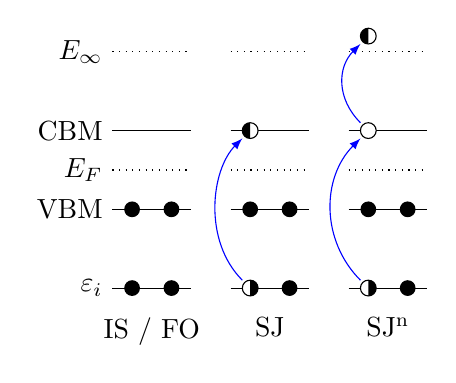
\begin{tikzpicture}
			\draw (0,0) node[left]{$\varepsilon_i$}-- node[midway,below=.25cm]{IS / FO} +(1,0);
			\draw (0,1) node[left]{VBM}-- +(1,0);
			\draw[dotted] (0,1.5) node[left]{$E_F$}-- +(1,0);
			\draw (0,2) node[left]{CBM}-- +(1,0);
			\draw[dotted] (0,3) node[left]{$E_\infty$}-- +(1,0);
			\fill (.25,0) circle (.1cm);
			\fill (.75,0) circle (.1cm);
			\fill (.25,1) circle (.1cm);
			\fill (.75,1) circle (.1cm);
			
			\begin{scope}[xshift=1.5cm]
				\draw (0,0) -- node[midway,below=.25cm]{SJ} +(1,0);
				\draw (0,1) -- +(1,0);
				\draw[dotted] (0,1.5) -- +(1,0);
				\draw (0,2) -- +(1,0);
				\draw[dotted] (0,3) -- +(1,0);
				\draw[fill=white] (.25,0) circle (.1cm);
				\fill (.25,-.1) arc (-90:90:.1);
				\fill (.75,0) circle (.1cm);
				\fill (.25,1) circle (.1cm);
				\fill (.75,1) circle (.1cm);
				\draw[fill=white] (.25,2) circle (.1cm);
				\fill (.25,1.9) arc (-90:-270:.1);
				\draw[-latex,blue] (.15,.1) .. controls +(-.5,.5) and +(-.4,-.4) .. (.15,1.9);
			\end{scope}
			
			\begin{scope}[xshift=3cm]
				\draw (0,0) -- node[midway,below=.25cm]{SJ\textsuperscript{n}} +(1,0);
				\draw (0,1) -- +(1,0);
				\draw[dotted] (0,1.5) -- +(1,0);
				\draw (0,2) -- +(1,0);
				\draw[dotted] (0,3) -- +(1,0);
				\draw[fill=white] (.25,0) circle (.1cm);
				\fill (.25,-.1) arc (-90:90:.1);
				\fill (.75,0) circle (.1cm);
				\fill (.25,1) circle (.1cm);
				\fill (.75,1) circle (.1cm);
				\draw[fill=white] (.25,2) circle (.1cm);
				\draw[-latex,blue] (.15,.1) .. controls +(-.5,.5) and +(-.5,-.5) .. (.15,1.9);
				\draw[-latex,blue] (.15,2.1) .. controls +(-.3,.3) and +(-.3,-.3) .. (.15,3.1);
				\draw[fill=white] (.25,3.2) circle (.1cm);
				\fill (.25,3.1) arc (-90:-270:.1);
			\end{scope}
		\end{tikzpicture}
		\caption{Approaches to compute BE's as the energy of the molecular orbital where the core hole is located: initial state (IS, also referred to as frozen orbitals, FO) and Slater-Janak (SJ) where the electron is put in the conduction band minimum (CBM). When the electron is further removed from the system (and conceptually pushed above the vacuum level, $E_\infty$), JS\textsuperscript{n} is noted. Adapted from Ref.~\citenum{pueyobellafontPredictingCoreLevel2017}.}
		\label{fig:method}
	\end{figure}
	
After the calculation, the corresponding eigenvalue, $\varepsilon_i\left(\frac{1}{2}\right)$, is extracted. The binding energy is then calculated as:
\begin{equation}
	\text{BE}_i = 
	E_{ref}- \varepsilon_i\left(\tfrac{1}{2}\right), \label{eq:xpsbe}
\end{equation}
where $E_{ref}$ is a reference energy, chosen to ensure consistency across systems. Different choices exist in the literature, and thus this study considers several choices for $E_{ref}$:
\begin{enumerate}
	\item $E_{ref}=0$, thus using only the orbital energy,
	\item $E_{ref}=E_F$, where the Fermi energy $E_F$ is used, 
	\item $E_{ref}=E_\infty$, the vacuum energy, calculated by taking the electrostatic potential in the vacuum region of the cell (when dipole correction are included, the vacuum potential is not equal on both sides of the slab, and therefore the average value is considered),
	\item $E_{ref}=\phi$, where the work function of the system $\phi = E_\infty - E_F$ is considered\cite{kahnFermiLevelWork2015}, and
	\item $E_{ref}= \varepsilon_{ref}$, where $\varepsilon_{ref}$ is the orbital energy of another atom in the cell. Although it might seem reasonable to use calcium, which is present in all slabs, this approach would depend on the slab's nature and would not be possible for gas-phase molecules. To overcome this, an Argon atom (to mimic calcium) is placed in the vacuum region, and $\varepsilon_{ref}=\varepsilon_{Ar,2s}$.
\end{enumerate}
Thus, computing a binding energy for a given atom requires to select a computational protocol, which includes the choice of a  way to deal with the electron reorganization  (in this work, SJ or SJ\textsuperscript{n}), and a $E_{ref}$.
It should, however, be noted that extracting $E_\infty$ is not feasible for bulk systems, where no vacuum region exists, or for charged systems, where the electrostatic potential is not constant in the vacuum region. This latter condition occurs when employing the SJ\textsuperscript{n} method. Nevertheless, it is possible to correct the Fermi level energy to remove the impact of the background of charge, as discussed in Ref.~\citenum{lozovoiInitioSimulationCharged2001}. This possibility is referred to as $E_{ref}=E_F'$, where $E_F' = E_F - \max\{E_{elst}(z)\}$, with $E_{elst}(z)$ being the planar average of the electrostatic potential along the $z$ axis. It is generally maximal in the center of the vacuum region.

Finally, while the determination of absolute binding energies (BE) is challenging from a theoretical perspective, the measurement or calculation of the work function, $\phi$ in Eq.~\eqref{eq:xps}, is also complex. As a result, both experimentalists and quantum chemists often focus on the relative binding energy, $\Delta\text{BE}$, which is the difference in binding energy for a given atom with respect  to that in a reference compound \cite{vinesPredictionCoreLevel2018,stevieIntroductionXrayPhotoelectron2020,greczynskiXrayPhotoelectronSpectroscopy2020}. In this contribution, relative BE values are computed as:\begin{equation}
	\Delta\text{BE}_i = \text{BE}_i - \text{BE}(\text{ref}), \label{eq:dbe}
\end{equation} 
using the calculated or experimental BE values for \ce{CH4}, \ce{NH3}, \ce{H2O}, \ce{B2H6}, and \ce{HF} as references for carbon, nitrogen, oxygen, boron, and fluorine, respectively. The experimental values are taken from Ref.~\citenum{pueyobellafontPredictingCoreLevel2017}. For calcium, the value for bulk Ca in CaO is used, taken from the XPS library \cite{cristXPSLibraryWebsite2021a} (computationally, a  2x2 slab containing 16 layers is used).

	
\section{Computational details}\label{sec:comp}

All calculations (geometry optimizations and binding energies) were performed  with VASP (version 6.4.1) using DFT with the PBE exchange-correlation functional, the D3 dispersion correction, and the projector-augmented wave (PAW) method.\cite{blochlProjectorAugmentedwaveMethod1994} The energy convergence criterion was set to \SI{e-4}{\electronvolt}, with a cutoff of \SI{550}{\electronvolt} for the kinetic energy of the plane waves. Gaussian smearing of the energy of valence electrons, with a width of \SI{0.2}{\electronvolt}, was applied.  Fermi energies were thus computed with \texttt{EFERMI = MIDGAP} in the VASP input. Brillouin zone integration was performed at the $\Gamma$-point for molecules in gas phase, using a 4x4x4 Monkhorst-Pack k-point mesh\cite{monkhorstSpecialPointsBrillouinzone1976} for bulk calculations, and a 4x4x1 mesh for slab calculations. The \texttt{Ca\_sv} pseudopotential\cite{blochlProjectorAugmentedwaveMethod1994,kresseUltrasoftPseudopotentialsProjector1999} was employed to model calcium.

\subsection{Geometry optimization} 
All optimizations were carried out using the Limited-memory Broyden-Fletcher-Goldfarb-Shanno  (L-BFGS) algorithm, driven by the Atomic Simulation Environment (ASE) package \cite{larsenAtomicSimulationEnvironment2017}, using VASP energies and forces as inputs, until the force on all atoms was below \SI{e-2}{\electronvolt\per\angstrom}.

In gas phase, each molecule was placed in a cubic box with a side length of \SI{20}{\angstrom} (with the molecule center of mass placed at the origin) and optimized (with frozen cell parameters).

In order to build slabs, bulk \ce{Ca^0} (from the Material Project, \texttt{MP-45}), CaO (\texttt{MP-2605}), and \ce{CaH2} (\texttt{MP-23713}) were selected, and their atomic positions and cell parameters were optimized. Subsequently, to determine the optimal surface orientation, 1x1 slabs with increasing thickness along different low-index orientations [(100), (110), and (111)] were constructed using ASE \cite{larsenAtomicSimulationEnvironment2017}. They have been constructed to ensure non-polar surfaces. The slabs were relaxed with the central two layers frozen to mimic bulk conditions, with the distance between slab repetitions set to 10 times the $c$ cell parameter of the bulk. For each orientation, the surface energy $\gamma^{hkl}$ was calculated by least-squares fitting of the following expression \cite{sunEfficientCreationConvergence2013,tranSurfaceEnergiesElemental2016}:
\begin{equation}
	E^{hkl}(N) = E_0\,N + 2A\,\gamma^{hkl} \label{eq:surf}
\end{equation}
where $N$ is the number of layers in the slab, $A$ is the slab surface area, $E^{hkl}(N)$ is the energy of the relaxed slab cut along $(hkl)$, and $E_0$ approximates the energy of one layer. The results (Table \ref{tab:surf}, Fig.~S2) indicate that (100) surfaces are the most energetically favorable, consistent with the literature \cite{deleeuwDensityFunctionalTheory2000,ebadiInsightsLiMetalOrganic2019}. 
Thus, using these (100) orientation, 3x3 (\ce{Ca^0} and CaO) and 2x2 (\ce{CaH2}) slabs (ensuring a slab surface of $\sim 10\times \SI{10}{\angstrom}$) consisting of 6 layers, with a vacuum of \SI{20}{\angstrom} between two slab repetitions were created and relaxed (with frozen cell parameters). 

Additionally, given that it was reported to be favorable\cite{deleeuwDensityFunctionalTheory2000,fujimoriInteractionWaterCaO2016a}, the adsorption of water on the CaO surface was investigated. In fact, the contamination of CaO by surface hydroxyls was reported in many experiments\cite{dupinSystematicXPSStudies2000,bebenseeAdsorptionOxygenWater2008,fujimoriInteractionWaterCaO2016a,cristXPSLibraryWebsite2021a}. Thus, an additional slab with full coverage (1 water molecule per surface Ca), denoted as \ce{CaO.H_2O}, was built and its geometry was also optimized. 

\begin{table*}
	\caption{Surface energies ($\gamma^{hkl}$, in \si{\joule\per\meter\squared}) of Ca, CaO, and \ce{CaH2} slabs along different orientations, as determined through Eq.~\eqref{eq:surf} using the $N$ values given in parentheses.}
	\label{tab:surf}
	\begin{ruledtabular}
	\begin{tabular}{lccc}
		
		&	\ce{Ca^0} & \ce{CaO} &	\ce{CaH2} \\
		\hline
		(100) & 0.555 ($N\in[6,16]$) & 0.470 ($N\in[6,16]$) & 0.871  ($N\in[12,32]$)\\
		(110) & 0.630  ($N\in[6,16]$)& 1.777  ($N\in[6,16]$)& 1.109 ($N\in[12,32]$)\\
		(111) & 0.563  ($N\in[6,16]$) & 4.080  ($N\in[5,15]$)  & 1.117   ($N\in[12,32]$) \\ 
		
	\end{tabular}
\end{ruledtabular}
\end{table*}

Finally, compounds \textbf{a}--\textbf{j} (Fig.~\ref{fig:THFdegradation}) were positioned on both sides of the slabs (to avoid the formation of surface dipole), initially placed approximately \SI{6}{\angstrom} from the surface. A final geometry optimization was then performed, keeping the cell parameters and the two central layers fixed.

\subsection{Binding energies} 

VASP allows targeting a specific orbital, $i$, by removing half an electron from it. For SJ calculation, dipole corrections (using the \texttt{IDIPOL} keyword) are included. For SJ\textsuperscript{n} calculations, it is necessary to adjust the total number of valence electrons (by default, half an electron is added, Fig.~\ref{fig:method}) using the \texttt{NELECT} keyword. Since it is not possible to account for spin-orbit coupling in such calculations, the study is limited to 1s and 2s binding energies. To simulate a spectrum, a Gaussian function centered at each computed \dbe{} is used. Unless otherwise specified, a full width at half maximum (FWHM) of \SI{0.5}{\electronvolt} is employed.

To evaluate the accuracy of the different computational protocols (SJ and SJ\textsuperscript{n} methods, as well as the choice of $E_{ref}$), two sets of calculations were conducted. First, the results from Pueyo Bellafont \textit{et al.} \cite{pueyobellafontPredictingCoreLevel2017}, which compare experimental and theoretical gas-phase \dbe{} values (computed at the same level of approximation as in this study, but with $E_{ref}=0$), were replicated. Their dataset includes 184 experimental absolute binding energies (BE's) from 68 molecules, covering carbon ($N=107$), nitrogen ($N=20$), oxygen ($N=22$), boron ($N=20$), and fluorine ($N=15$) atoms (see the supplementary material, Fig.~S1). Each molecule was placed in a cubic box with a side length of \SI{20}{\angstrom}, centered at the molecule's center of mass. The \dbe{} values were then computed for each atom of interest. Other parameters, such as vacuum energy, were extracted from the density (\texttt{CHGCAR}) and potential (\texttt{LOCPOT}) files. For calculations involving an additional argon atom, it was positioned at the center of the box.

In parallel, the effect of slab thickness was examined using the bare slabs of increasing thickness described above. Binding energies were calculated on 2x2 slabs with a (100) orientation, separated by an interslab distance of \SI{20}{\angstrom}. The geometries were based on the optimized 1x1 slabs from the surface energy study, with a supercell created and then adjusting the interslab spacing. The \dbe{} values were computed for each atom of interest, and the relevant parameters were extracted accordingly. For calculations involving an additional argon atom, placed in a cell where the slab is positioned at the center, it was located at the origin.

Finally, the \dbe{} values were calculated for each atom of interest in the molecules grafted onto the various surfaces, using the selected reference energy. It is important to note that, in these calculations with the SJ protocol, the relatively small surface area of the slabs could introduce artifacts due to the periodic repetition of core holes in close proximity, especially for adsorbates that are far from the surface.\cite{taucherFinalStateSimulationsCoreLevel2020} This is however partially mitigated when reporting relative rather than absolute BE's and using dipole corrections. Furthermore, although larger supercells could be employed to mitigate this issue, doing so would significantly increase computational time.

\clearpage



\section{Results}\label{sec:results}

\NewDocumentCommand{\cpx}{O{}m}{SJ\IfNoValueTF{#1}{}{\textsuperscript{#1}}+$E_{ref} = #2$}

\subsection{Selection of a computational protocol for binding energies}\label{sec:proto}

\subsubsection{Molecules in gas phase}

A comparison between experimental and computed \dbe{} values for carbon is shown in Fig.~\ref{fig:xps_C185_C}. Within the SJ\textsuperscript{n} approach, consistent with previous studies \cite{pueyobellafontPredictingCoreLevel2017,golzeAccurateAbsoluteRelative2020}, the \cpx[n]{0} protocol provides reliable results for all atoms, exhibiting a very small mean error and an acceptable standard deviation. However, achieving this level of agreement requires using a reference per atom (Table S1), since the difference between experimental and computed absolute BE's increases with the atomic number. Similarly, using \cpx[n]{\varepsilon_{Ar,2s}} protocol results in small errors, which is consistent with the observation of Garcià-Gil \textit{et al.}\cite{garcia-gilCalculationCoreLevel2012} (although they only used IS calculations). Across the entire set of 184 \dbe{} values, the combination of either $E_{ref}=0$ or $E_{ref}=\varepsilon_{Ar,2s}$ with the SJ\textsuperscript{n} approach yields comparable results (Fig.~\ref{fig:xps_C185}). In contrast, other reference energies significantly degrade the accuracy of the predicted gas-phase \dbe{}. The largest errors are observed when using the Fermi energy \cpx[n]{E_F}, or \cpx [n]{E_F'}, and it leads to underestimated \dbe{} values. 

Turning more specifically to the SJ approach, \cpx{E_F} also gives large errors, then \cpx{0}, \cpx{\varepsilon_{Ar,2s}}, and \cpx{E_\infty} perform similarly, and finally, the lowest error found when using \cpx{\phi}, although it remains substantial. Moreover, all reference energies combined with the SJ protocol tend to overestimate the \dbe{} values. One possible reason is that placing a (half) electron in the LUMO of a molecule significantly alters its electronic structure (Fig.~S3), often more so than the interaction of the core-hole itself, which appears to be better captured by the SJ\textsuperscript{n} approach.\cite{taucherFinalStateSimulationsCoreLevel2020}


\begin{figure*}
	\centering
	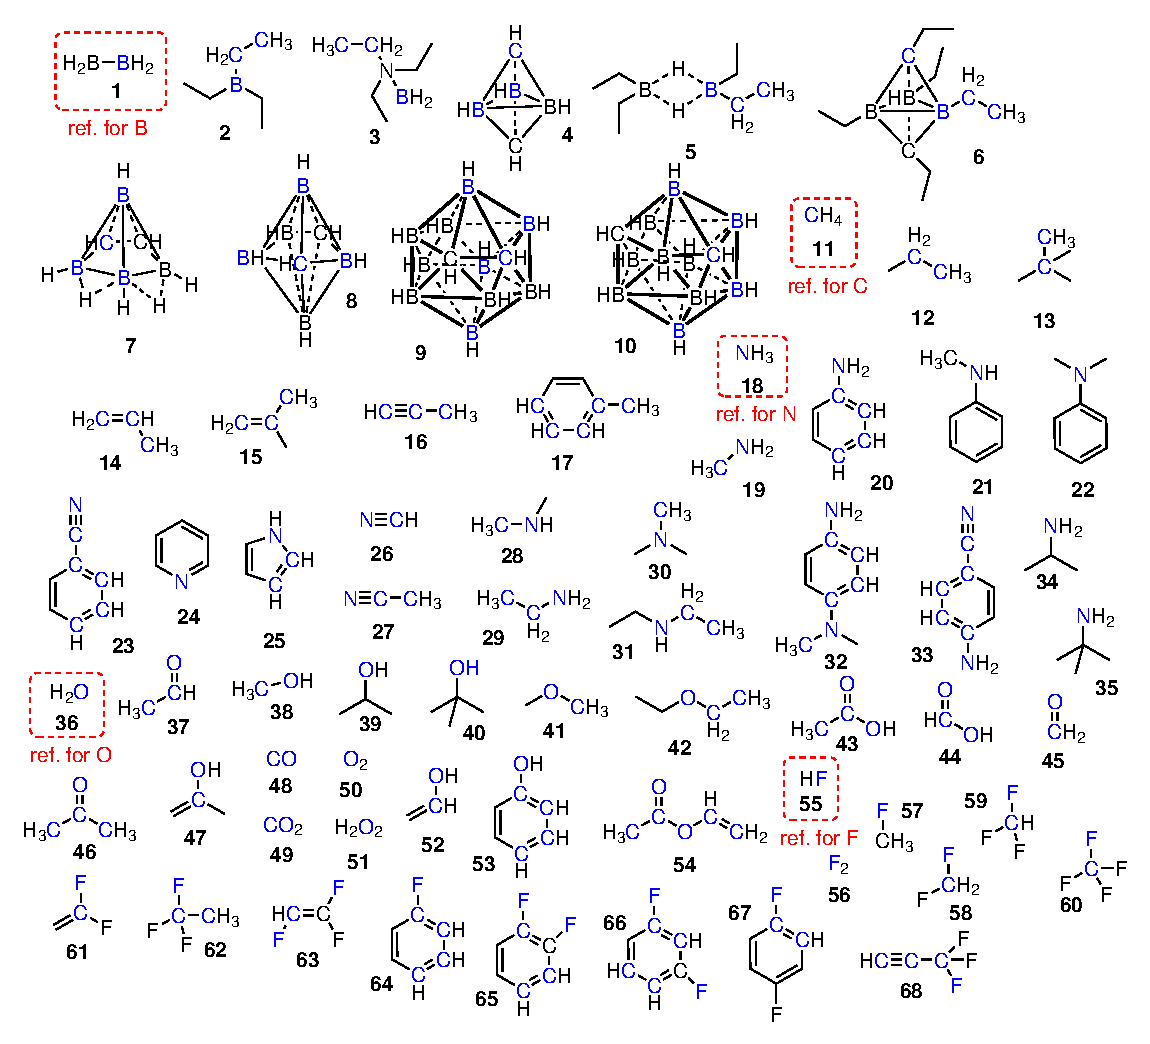
\includegraphics[width=\linewidth]{Figure3}
	\caption{Error in the calculated gas-phase \dbe{}  (in \si{\electronvolt}) with respect to experiment, computed using the SJ (panel a) and SJ\textsuperscript{n} (panel b) method and different reference energies, for the carbon atom ($N=107$). For each reference, the violin plot illustrates the error distribution (horizontal lines represent, from bottom to top, the minimum, 1\textsuperscript{st} quartile, median, 3\textsuperscript{rd} quartile, and maximum). Additionally, the mean $\pm$ standard deviation values are displayed}
	\label{fig:xps_C185_C}
\end{figure*}


\begin{figure}[p]
	\centering
	\includegraphics[width=.8\linewidth]{Figure4}
	\caption{Comparison between experimental and calculated gas phase \dbe{} (in \si{\electronvolt}), as computed with the two best-performing protocols, on the different atoms (panels a-e). For each of them, the error (as mean $\pm$ standard deviation) is given.}
	\label{fig:xps_C185}
\end{figure}

\clearpage

\subsubsection{Bare slabs}

The situation differs for the bare slabs. The impact of slab thickness ($N$) on the Ca 2s binding energy, evaluated using both protocols, is shown in Figs.~\ref{fig:slabsthicknessSJ}-\ref{fig:slabsthicknessSJn}. The results reveal a substantial difference (exceeding \SI{0.5}{\electronvolt} for certain reference energies) between the surface layers (defined as the first and last layers of the slab) and the bulk \dbe{}. With all protocols, BE(surface Ca 2s) $>$ BE(bulk Ca 2s). The difference between bulk and surface BE's are referred to as surface core level shifts (SCLS),\cite{olovssonCorelevelShiftsComplex2006,bagusChemicalSignificanceXray2023} which have been reported for metals\cite{aldenInitioSurfaceCorelevel1993,weinertCorelevelShiftsBulk1995,olovssonCorelevelShiftsComplex2006} and oxides\cite{harmerSpeciesFormedCuprite2009,lousadaFirstStagesOxide2018,bagusRevisitingSurfaceCorelevel2019,cristinadeoliveiraRoleSurfacesMagnetic2021,silvalucenademedeirosAMoO3MicroNanoparticles2024}. One of the main cause of this difference is the change in Madelung energy between the bulk and surface atoms\cite{nelinSurfaceCorelevelBinding2014}, though this is not the only effect\cite{bagusRevisitingSurfaceCorelevel2019,bagusChemicalSignificanceXray2023,bagusXrayPhotoelectronSpectroscopy2024}. 
Note that these figures also display the standard deviation ($\sigma$), which measures the variation of BE's within bulk and surface values (Figs.~S4-S5). For the surface layer, this standard deviation is expected to be small, as all atoms are in a similar environment, while it is moderate for bulk values (here, it is generally $<\SI{0.1}{\electronvolt}$) due to differences in atomic environments based on $z$-position. The standard deviation should also increase with the number of layers ($N$). However, for certain calculations, particularly those with $E_{ref}=\varepsilon_{Ar,2s}$ (and some other methods using the thickest slabs), the variation becomes significant and disrupts the expected trends. Values of mean BE's with $\sigma > \SI{0.5}{\electronvolt}$, which appears erroneous, were therefore excluded from the graphs.


Another key observation is that slab thickness influences some results more than others. For calculations with \cpx{E_F}, \cpx[n]{E_F}, \cpx{\varepsilon_{Ar,2s}}, and \cpx{E_\infty}, the predicted values remain nearly constant as $N$ increases. Conversely, other protocols (such as \cpx{0}, \cpx[n]{0}, \cpx{\phi}, or \cpx[n]{E_F'}) appear very sensitive to the system size. 

For O 1s, as illustrated in Fig.~\ref{fig:slabOH2}, where simulated XPS spectra for CaO and \ce{CaO.H2O} (both with 6 layers) are shown  (values are also provided in Tables S2-S3), the distinction between bulk and surface contributions is noticable. In the case of CaO, BE(bulk O 1s in CaO) $\geq$ BE(surface O 1s in CaO), whereas in \ce{CaO.H2O}, the reverse trend is observed, consistent across all protocols. Furthermore, BE(bulk O 1s in CaO) $\approx$ BE(bulk O 1s in \ce{CaO.H2O}) (difference of \SI{0.2}{\electronvolt} or smaller) when using \cpx{E_F}, \cpx{E_\infty}, \cpx[n]{E_F}, or \cpx{\varepsilon_{Ar,2s}}. However, the latter yields unreliable results, as evidenced by the spurious peak at \dbe{} = \SI{0}{\electronvolt} in the O 1s spectra, suggesting an artificial differentiation between hydroxyl environments that is not reflected when using other reference energies. Finally,  BE(surface O 1s in \ce{CaO.H2O}) $\geq$ BE(hydroxyl O 1s  in \ce{CaO.H2O}), but the difference ranges from 0 (\textit{e.g.}, \cpx{E_\infty}) to \SI{0.5}{\electronvolt} (\cpx[n]{E_F'}). This latter results was also found by Fujimori \emph{et al.} \cite{fujimoriInteractionWaterCaO2016a} via calculations using a similar method to ours (and \cpx{E_\infty}), which also showed that the separation between these two BE's depends on the hydroxyl coverage of the surface.



\begin{figure}[p]
	\centering
	\includegraphics[width=\linewidth]{Figure5}
	\caption{Effect of slab thickness (expressed as the number of layers, $N/N_0$, where $N$ is the number of layers in the slab while $N_0 = 2$ for \ce{Ca^0} and CaO and 4 for \ce{CaH2} represents the number of layers in the unit cell)  on the mean bulk (filled markers) and surface (empty markers) \dbe{} for Ca 2s (in \si{\electronvolt}), calculated using the SJ method and various reference energies (panels a-e). The vertical lines indicate the standard deviation of BE's  (generally not visible because very small). See text for missing value at $N/N_0=8$.}
	\label{fig:slabsthicknessSJ}
\end{figure}

\begin{figure}[p]
	\centering
	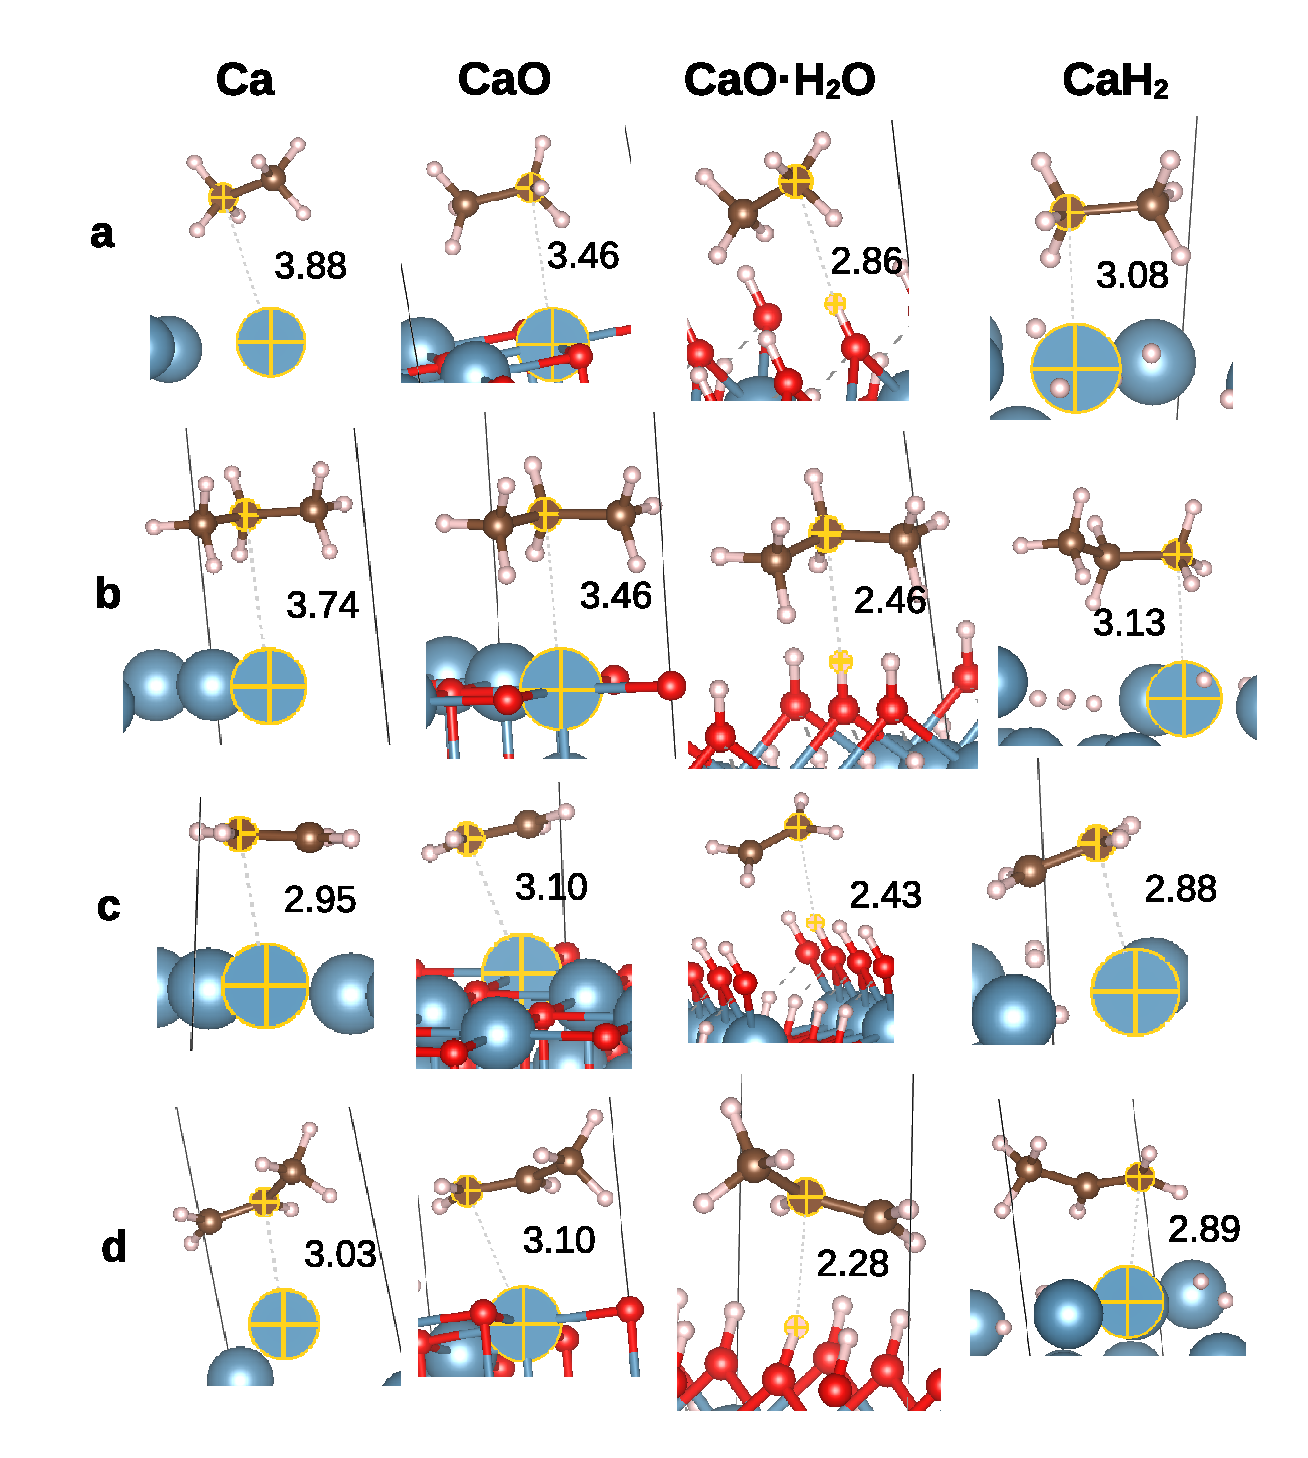
\includegraphics[width=\linewidth]{Figure6}
	\caption{Effect of slab thickness (expressed as the number of layers, $N/N_0$, where $N$ is the number of layers in the slab while $N_0 = 2$ for \ce{Ca^0} and CaO and 4 for \ce{CaH2} represents the number of layers in the unit cell)  on the mean bulk (filled markers) and surface (empty markers) \dbe{} for Ca 2s (in \si{\electronvolt}), calculated using the SJ\textsuperscript{n} method and various reference energies (panels a-d). The vertical lines indicate the standard deviation of BE's (generally not visible because very small).}
	\label{fig:slabsthicknessSJn}
\end{figure}


\begin{figure}[p]
	\centering
	\includegraphics[width=\linewidth]{Figure7a}
	\includegraphics[width=\linewidth]{Figure7b}
	\caption{Effect of the reference energy on the simulated Ca 2s (panels a and c)  and O 1s (panels b and d) XPS spectra of CaO (dashed line)  and \ce{CaO.H2O} (plain line), calculated using the different protocols (panels a-b and c-d). Letters indicate mean values for bulk (``b"), surface (``s"), and surface hydroxides (``h", only for \ce{CaO.H2O}  O 1s).}
	\label{fig:slabOH2}
\end{figure}

Experimentally, XPS spectra for calcium metal slabs and their oxides, including Ca 2s binding energies, are scarce. Some values from various sources are summarized in Table S4. To the best of our knowledge, no reported measurements exist for \ce{CaH2}, and data for other peaks are limited \cite{franzenXPSSpectraCrystalline1977,sveinbjornssonIonicConductivityFormation2014}. Moreover, due to calcium's high reactivity, contamination by oxides, hydroxyls, and hydrocarbons complicates the analysis \cite{dupinSystematicXPSStudies2000,bebenseeAdsorptionOxygenWater2008,fujimoriInteractionWaterCaO2016a,cristXPSLibraryWebsite2021a}. Nonetheless, two trends can be discerned: \begin{inparaenum}[(i)]
	\item unlike the preceding alkaline earth metal, magnesium \cite{dobrovolskyXPSStudyInfluence2017}, recent data suggest that BE(Ca 2s in \ce{Ca^0}) $>$ BE(Ca 2s in CaO) $\approx$ BE(Ca 2s in \ce{CaO.H2O}) \cite{ochsCO2ChemisorptionCa1998,cristHandbookMonochromaticXPS2000a,cristXPSLibraryWebsite2021a}, and 
	\item BE(Bulk O 1s in CaO) $\approx$ BE(bulk O 1s in \ce{CaO.H2O}) $<$ BE(hydroxyls O 1s in \ce{CaO.H2O}) \cite{dupinSystematicXPSStudies2000,bebenseeAdsorptionOxygenWater2008,fujimoriInteractionWaterCaO2016a,cristXPSLibraryWebsite2021a}.
\end{inparaenum}
Only the \cpx{E_\infty} protocol satisfies these two criteria, and provide the correct trends. Consequently, a consistent treatment of both gas-phase systems and slabs using the same method is not feasible in this work. Also note that this protocol globally underestimates the \dbe{} for O 1s (which is, \textit{e.g.}, smaller than \SI{-7}{\electronvolt} for bulk CaO\cite{cristXPSLibraryWebsite2021a}). Finally, Bagus \emph{et al.}\cite{bagusRevisitingSurfaceCorelevel2019} also argued recently that the difference between bulk and surface O 1s in CaO, which amounts to \SI{0.5}{\electronvolt} with this protocol, is overestimated  and should be $<\SI{0.1}{\electronvolt}$.



\clearpage

\subsection{Adsorption on slab: geometrical and energetic aspects}\label{sec:geom}

The optimized geometries of compounds \textbf{a}-\textbf{j}, following their adsorption on each side of the slabs, are depicted in Figs.~\ref{fig:distsad}-\ref{fig:distsj}. The interaction energy, calculated as $\Delta E_{int} = E_{2X@Y} - E_Y - 2E_X$ (where $E_X$ represents the energy of a single adsorbate, in gas phase, and $E_Y$ is the energy of the neat substrate), is presented in Table~\ref{tab:int}. Note that no thermochemical corrections (i.e., zero-point vibrational energy and thermal corrections) have been applied in these calculations.

\begin{figure}[!b]
	\centering
	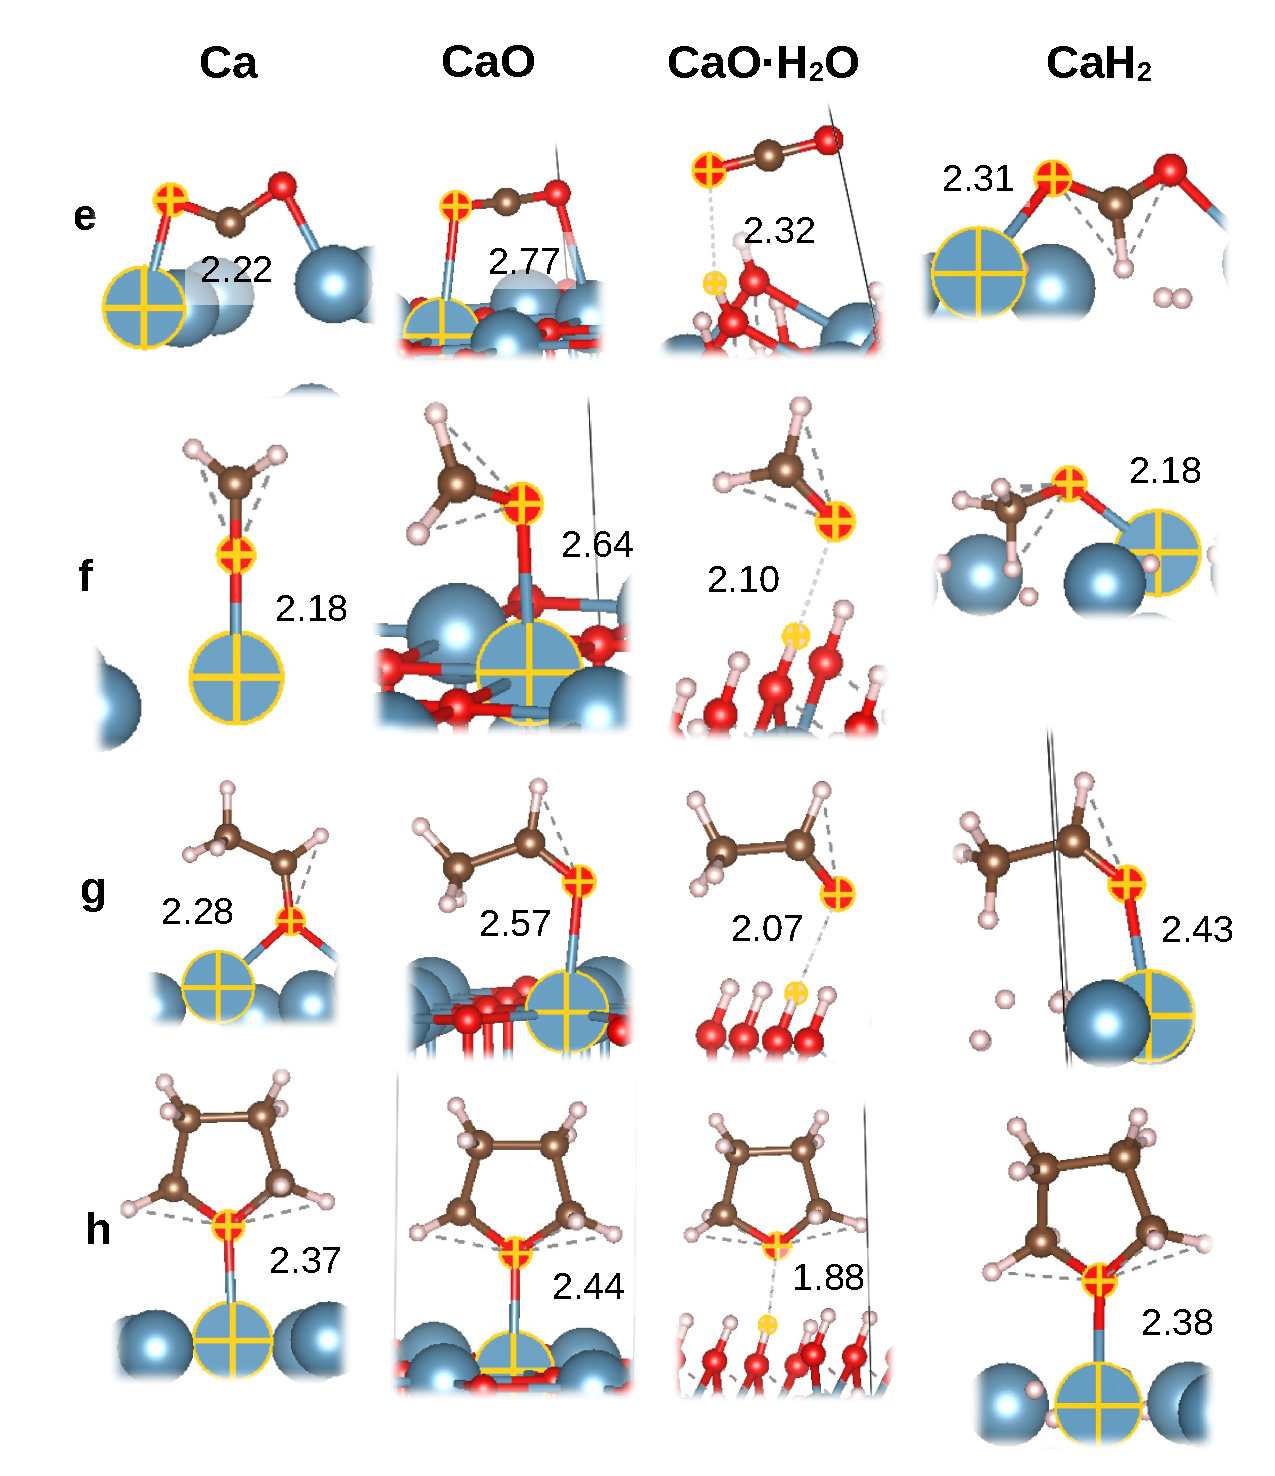
\includegraphics[width=\linewidth]{Figure8}
	\caption{Geometrical structures of the adsorbate (hydrocabrons, \textbf{a}-\textbf{d}) + substrate systems, after geometry optimization, described by representative intermolecular distances (in \si{\angstrom}).}
	\label{fig:distsad}
\end{figure}

\begin{figure}[!h]
	\centering
	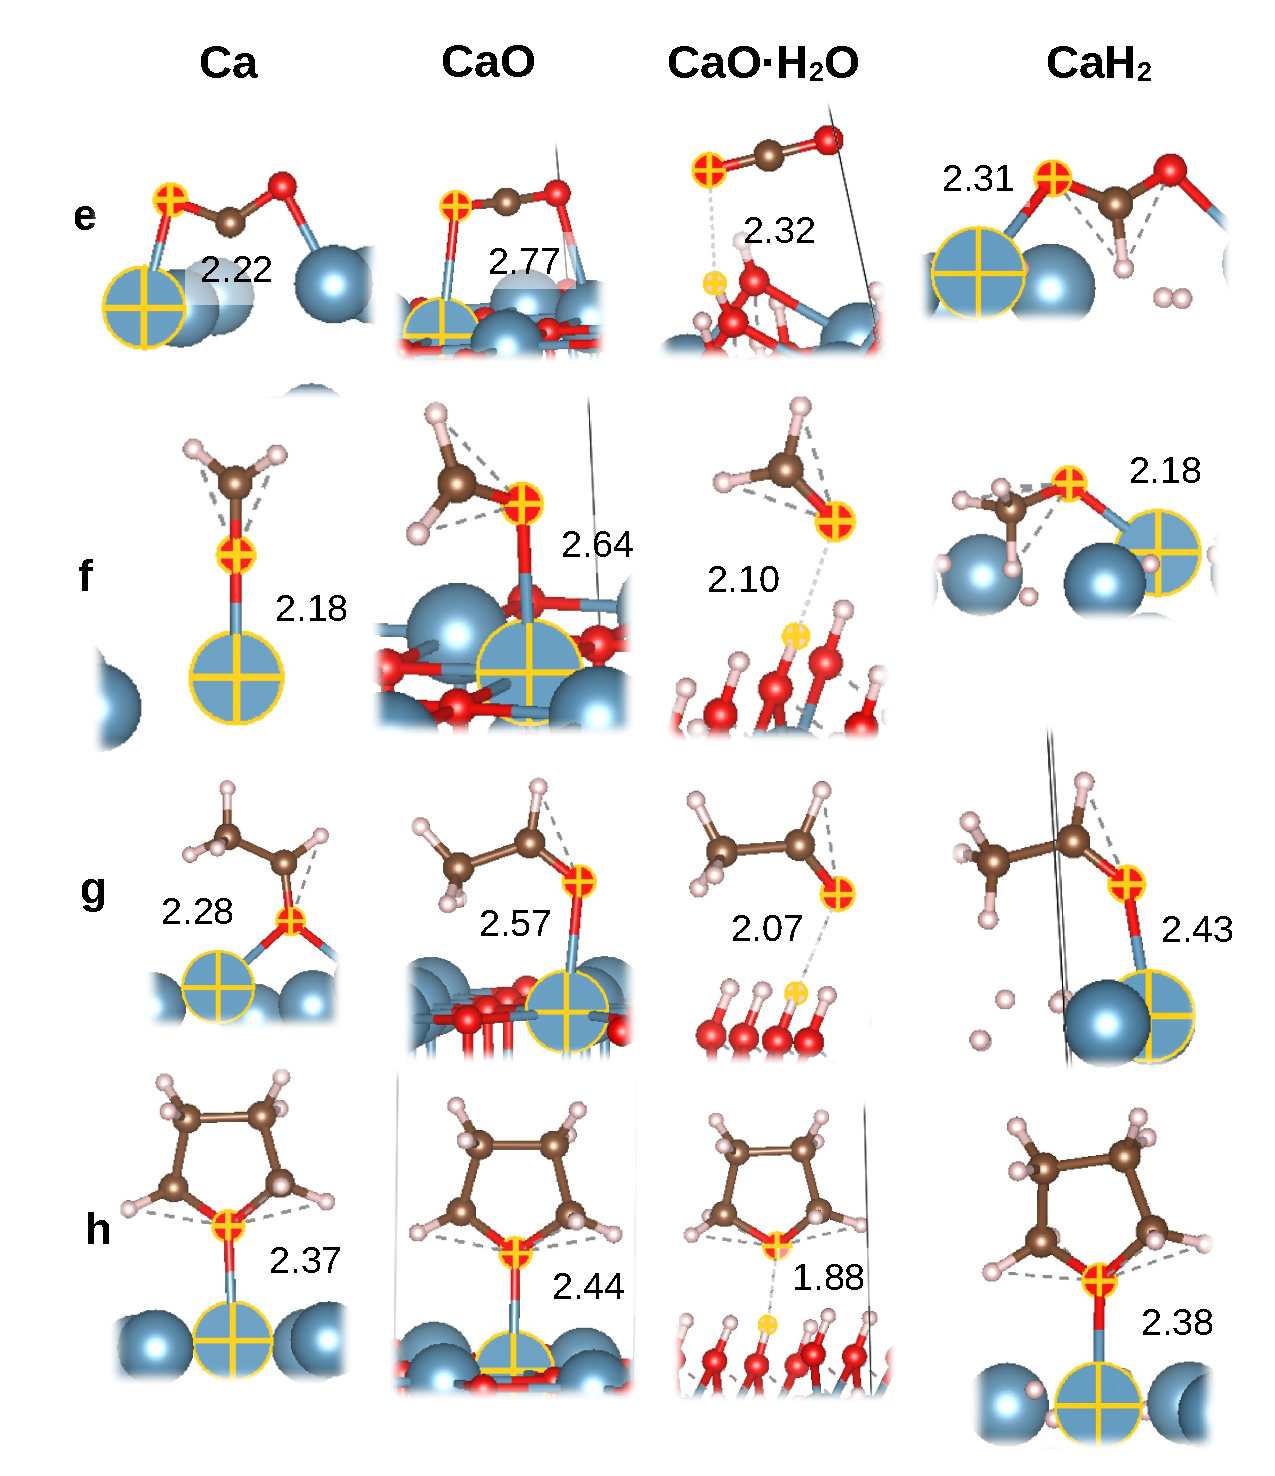
\includegraphics[width=\linewidth]{Figure9}
	\caption{Geometrical structures of the adsorbate (aprotic polar molecules, \textbf{e}-\textbf{h}) + substrate systems, after geometry optimization, described by representative intermolecular distances (in \si{\angstrom}).}
	\label{fig:distsei}
\end{figure}

\begin{figure}[!h]
	\centering
	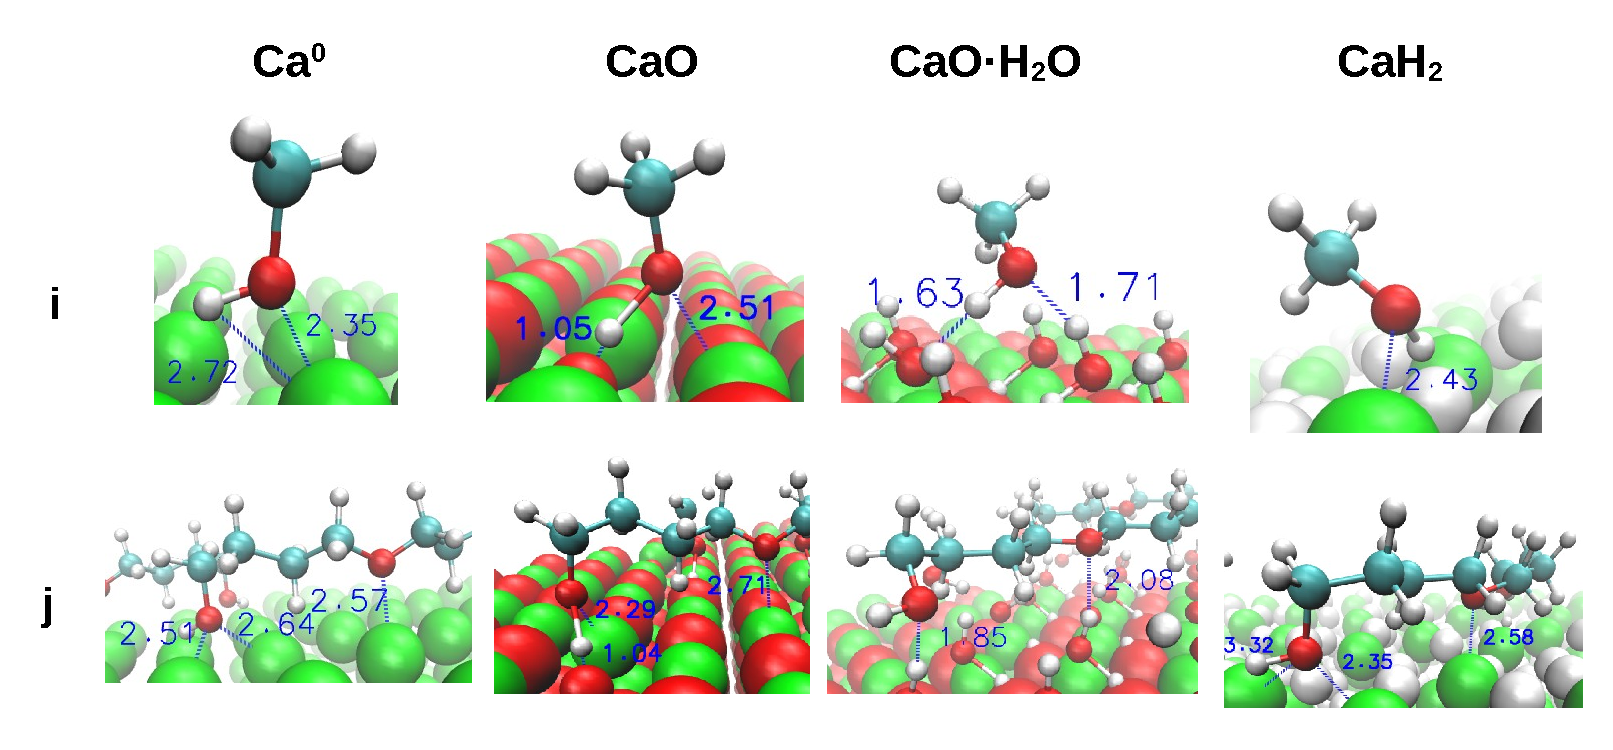
\includegraphics[width=\linewidth]{Figure10}
	\caption{Geometrical structures of the adsorbate (protic miolecules, \textbf{i}-\textbf{j}) + substrate systems, after geometry optimization, described by representative intermolecular distances (in \si{\angstrom}).}
	\label{fig:distsj}
\end{figure}

\begin{table}[!h]
	\caption{Interaction energy ($\Delta E_{int}$, in \si{\electronvolt}) between the adsorbate and the substrate.}
	\label{tab:int}
	\begin{ruledtabular}
	\begin{tabular}{>{\bfseries}lcccc}
		& Ca & \ce{CaO} & \ce{CaO.H2O} & \ce{CaH2} \\
		\hline
		& \multicolumn{4}{c}{Hydrocarbons} \\
		a & -0.67 & -0.44 & -0.65 & -0.41 \\
		b & -0.42 & -0.63 & -0.87 & -0.52 \\
		c & -0.95 & -0.34 & -0.78 & -0.80 \\
		d & -1.04 & -0.53 & -0.98 & -0.84 \\
		\hline
		& \multicolumn{4}{c}{Polar molecules} \\
		e & -2.03 & -0.37 & -0.67 & -6.42 \\
		f & -3.21 & -0.41 & -0.97 & -1.99 \\
		g & -1.52 & -0.70 & -1.18 & -2.72 \\
		h & -1.62 & 2.08 & -1.31 & -1.61 \\
		\hline
		& \multicolumn{4}{c}{Protic molecules} \\
		i & -1.81 & -1.60 & -2.19 & -1.64 \\
		j & -4.53 & -2.54 & -5.60 & -4.31 \\
	\end{tabular}
\end{ruledtabular}
\end{table}

\clearpage

There are three primary modes of interaction between the substrate and the adsorbate: \begin{inparaenum}[i)] \item van der Waals (vdW) forces, 
\item hydrogen bonding (HB), and 
\item chemisorption. 
\end{inparaenum}
First, hydrocarbons (\textbf{a}–\textbf{d}) mainly interact through vdW forces, as indicated by the relatively large distances between the adsorbate and substrate (Fig.~\ref{fig:distsad}) and the low interaction energies ($\Delta E_{int} > \SI{-1}{\electronvolt}$). However, for unsaturated hydrocarbons (\textbf{c}-\textbf{d}), the distances are shorter ($\sim\SI{3}{\angstrom}$) compared to saturated ones (\textbf{a}-\textbf{b}) on the \ce{Ca^0} and \ce{CaH2} slabs, leading to slightly higher interaction energies.

Second, HB interactions are significant between \ce{CaO.H2O} and oxygen-containing mole\-cules (\textbf{e}-\textbf{j}). For non-protic molecules (\textbf{e} to \textbf{h}), interaction energies decrease (\textit{i.e.}, the binding is stronger) as the oxygen(substrate)--hydrogen(slab) distance decreases (up to $\Delta E_{int}<\SI{-1.3}{\electronvolt}$ for \textbf{h}), with the molecule's oxygen acting as the HB donor. For protic molecules (\textbf{i} and \textbf{j}), additional HB interactions form between the substrate hydrogen and slab oxygens. The multiplication of slab-substrate HB interactions correlates with a further increase of the interaction energies (in absolute value).


Lastly, oxygen-containing molecules can exhibit significant interaction energies ($\Delta E_{int} < \SI{-1.5}{\electronvolt}$) with the \ce{Ca^0} and \ce{CaH2} slabs, primarily driven by strong oxygen--calcium interactions. These are often accompanied by small interatomic distances, indicative of chemisorption. This effect is particularly pronounced for PTMEG (\textbf{j}), where multiple interactions account for the large interaction energy. Similarly, \ce{CO2} (\textbf{e}) and \ce{CH2=O} (\textbf{f}) display notable interactions with the \ce{CaH2} slab. Note that for \ce{CO2}, two binding configurations are possible (Fig.~\ref{fig:distsei}), with the reported interaction energy representing the sum of the contributions from both configurations. These cases are distinguishable by their difference of hybridization (\textit{e.g.}, from \ce{sp^2} to \ce{sp^3} for \textbf{f}). These transformations are facilitated by interactions with a slab’s hydrogen atoms.

Interestingly, the \ce{CaO} slab exhibits a distinct trend. Interactions with polar molecules (\textbf{e}-\textbf{h}) yield low interaction energies, comparable to van der Waals forces, or even positive values in the case of \textbf{h}. For protic molecules (\textbf{i}-\textbf{j}), while HB accounts for some of the slab-substrate interactions, the small hydrogen(substrate)--oxygen(slab) distances observed suggest the occurrence of proton transfer between the substrate and the slab.

These observations provide insights into potential degradation mechanisms involving these molecules. The proton transfers to the CaO surface support the hypothesis of hydroxyl formation on the slab. Moreover, reactions involving hydrogen from the \ce{CaH2} slab indicate possible surface reactivity under certain conditions.  It should be noted that these reactions are not necessarily associated with an important modification of the slab structure, as measured by the mean displacements of the calcium atoms after adsorption (Table S5). In fact, \ce{CaH2} tends to be the most affected by adsorption, regardless of the adsorbate.

%\clearpage
\subsection{Binding energies of adsorbate on slabs}\label{sec:BE's}

\newcommand{\XPSsa}[2]{
	\begin{figure}[!h]
		\centering
		\includegraphics[width=\linewidth]{Figure#1}
		\caption{Difference (dotted line) between the XPS spectra before (dashed line) and after (solid line) adsorption for compounds \textbf{#2} on various substrates, as computed using the \cpx{E_\infty} protocol. Letters indicate mean binding energies for bulk (``b"), surface (``s", with $\star$ marking the atom closest to the adsorbate), surface hydroxides (``h"), and different atoms of the adsorbate.}
		\label{fig:spectraXPSads#2}
	\end{figure}
}

\newcommand{\XPSsab}[4]{
	\begin{figure}[p]
		\centering
		\includegraphics[width=\linewidth]{Figure#1}
		\includegraphics[width=\linewidth]{Figure#2}
		\caption{Difference (dotted line) between the XPS spectra before (dashed line) and after (solid line) adsorption for compounds \textbf{#3} (panel a) and \textbf{#4} (panel b) on various substrates, as computed using the \cpx{E_\infty} protocol. Letters indicate mean binding energies for bulk (``b"), surface (``s", with $\star$ marking the atom closest to the adsorbate), surface hydroxides (``h"), and different atoms of the adsorbate.}
		\label{fig:spectraXPSads#3#4}
	\end{figure}
}

Directly comparing binding energies (BE's) of molecules in the gas phase with those adsorbed on a slab is methodologically problematic (as discussed \textit{vide supra}). Therefore, the focus here will be on the binding energies before (slab) and after (slab + adsorbate) adsorption.
The spectra corresponding to the adsorption of compound \textbf{a} (Fig.~\ref{fig:spectraXPSadsac}a) is first analyzed. Adsorption induces a slight shift in the bulk BE's (labeled ``b"), which ideally should remain unaffected. While using thicker slabs could mitigate this issue, the discussion  focuses on the surface BE's (labeled ``s"), which exhibit the most significant adsorption-induced changes. In this example, the surface calcium and oxygen atoms closest to \textbf{a} (labeled ``s$^\star$") show similar BE values before and after adsorption, consistent with weak van der Waals (vdW) interactions and large substrate-adsorbate distances. Additionally, a peak corresponding to the carbon of \textbf{a} is observed around $\dbe = \SI{0}{\electronvolt}$, characteristic of a saturated carbon. The spectra for compound \textbf{b} (Fig.~S6a) are quite similar, though the carbon peak is larger due to the slightly different BE's of \ce{-CH3} and \ce{-CH_2-} groups, with the latter showing a higher BE.


Next, the spectra of compound \textbf{c} (Fig.~\ref{fig:spectraXPSadsac}b) is analyzed. In this case, the surface calcium atoms in close contact with the adsorbate (labeled ``s$^\star$") experience a shift towards lower BE's (sometimes accompanied by other surface atoms,  labeled ``s''). No significant changes are observed in the oxygen atoms, whose BE values remain consistent with the previous spectra. In comparison to \textbf{a}, a distinct peak corresponding to the unsaturated carbon atoms appears around $\dbe = \SI{-1}{\electronvolt}$. This peak also show that the distance between the adsorbate and the surface can have an impact (here, the larger the distance, the smaller \dbe{}), as reported by Taucher \emph{et al.}\cite{taucherFinalStateSimulationsCoreLevel2020}. The spectra for compound \textbf{d} (Fig.~S6b) show a similar trend, with a separate peak for each type of carbon.

\XPSsab{11a}{11b}{a}{c}

\clearpage

Turning to compound \textbf{e} (Fig.~\ref{fig:spectraXPSadse}), several notable features arise, as reactions occur between \ce{CO2} and the \ce{Ca^0} and \ce{CaH2} slabs. In the latter, these interactions affect the oxygen spectra, resulting in two distinct peaks, as there are two distinct cases (Fig.~\ref{fig:distsei}): one associated with one of the oxygens of a quasi-$D_{\infty h}$ \ce{CO2} molecule  (around $\dbe = \SI{1}{\electronvolt}$, labeled ``linear''), and another associated with a bent $C_{2v}$-like \ce{CO2} molecule (around $\dbe = \SI{-2}{\electronvolt}$, labeled ``bent''), which arises from the reaction. The relative intensities of these peaks depend on the composition and coverage of the slab, which were not investigated in this study.\cite{dahleSituPreparationCalcium2012,fujimoriInteractionWaterCaO2016a} The other O 1s spectra present one or the other peak, depending on the slab-substrate interaction. The same goes for the C 1s spectra, the C atom of the linear and bent \ce{CO2} molecules gives rise to peaks located around $\dbe = \SI{3.5}{\electronvolt}$ and $\dbe = \SI{1.5}{\electronvolt}$, respectively, but with some variability for this last peak: interaction between \ce{CO2} and an hydrogen of \ce{CaH2} leads to a larger BE's (at \SI{1.8}{\electronvolt}) than interaction with Ca in \ce{Ca^0} (at \SI{0.9}{\electronvolt}). Finally, surface calcium are also affected, which results in changes in Ca 2s spectra, particularly with \ce{CaH2}. Surprisingly, it does not affect much the spectrum for \ce{Ca^0}.

The results of O 1s are in line with previous studies by Maus-Friedrichs and colleagues\cite{ochsCO2ChemisorptionCa1998,voigtsAdsorptionCO2CO2009,dahleSituPreparationCalcium2012}, which investigated the adsorption of \ce{CO2} on \ce{Ca^0} and \ce{CaO}, showing the formation of a calcite layer. Their most recent experimental XPS data\cite{dahleSituPreparationCalcium2012} indicate that BE(O 1s in \ce{CO3^-}) is higher than BE(bulk O 1s in CaO) by approximately \SI{3}{\electronvolt}, a trend similar to that observed in this study, although the present case concerns \ce{CO2}. Preliminary calculations on \ce{CaCO3} (not shown here) further support this trend. 

The spectra for compounds \textbf{f} and \textbf{g} (Fig.~S7) exhibit similar trends. However, the carbon in compound \textbf{f} undergoes a transition from a planar $C_{2v}$-like geometry to a triangular pyramid (resembling a $C_{3v}$ symmetry, though there is one C-O bond and two C-H bonds) upon reacting with \ce{CaH2}, and thus the peaks appear at lower \dbe{}. Additionally, the strong interaction between the oxygen atoms in compounds \textbf{f} and \textbf{g} and the \ce{Ca^0} substrate results in a notable shift towards lower \dbe{} values in both the O 1s and C 1s spectra.  A notable shift in the Ca 2s results for \ce{CaO.H2O} slab is also noted, associated with the thickness of the slab.

\XPSsa{12}{e}
\clearpage

Finally, the spectra of THF and its short model polymer (Fig.~\ref{fig:spectraXPSadshj}) are analyzed together. The main observations are: \begin{inparaenum}[(i)]
	\item the peak with associated to the ether moiety in both molecules is associated to large BE's (around \SI{0}{\electronvolt} in O 1s, where it is labeled ``\ce{O-C}", and around \SI{1.5}{\electronvolt} for C 1s, labeled ``\ce{C-O}"), 
	\item for compound \textbf{j}, a second peak with lower BE's is associated to the presence of alcohol moieties (around \SI{-1}{\electronvolt} in O 1s, where it is labeled ``\ce{OH-C}", and around \SI{1.5}{\electronvolt} for C 1s, labeled ``\ce{C-OH}"), 
	\item cyclization slightly affects the peak associated with saturated carbons (labeled ``\ce{C-C}") towards larger values, and
	\item when grafted on CaO, proton transfer between PTMEG (\textbf{j}) and surface leads to a shift of about \SI{-2}{\electronvolt}  (thus similar to the value for compounds \textbf{f}) in the O 1s spectrum and of about \SI{0.7}{\electronvolt} in C 1s (again, becoming similar to compound \textbf{f}). This is also the case for compound \textbf{i} (Fig.~S8).
\end{inparaenum}

\XPSsab{13a}{13b}{h}{j}

\clearpage

The trends across all spectra are summarized in Fig.~\ref{fig:trends}. Given the low sensitivity of the Ca 2s core level to environmental changes, it has been excluded from the analysis. The binding energy (BE) values for C 1s and O 1s exhibit a clear correlation with the hybridization state of the atoms and the electronegativity of their neighboring atoms, as anticipated.\cite{stevieIntroductionXrayPhotoelectron2020} 
Key findings of this study are also summarized in this last figure, which include: 
\begin{inparaenum}[(i)]
	\item the pronounced effect of oxygen-calcium interactions on the BE, highlighted by the red bars for C 1s values and also evident in the distinction between ``OH-C'' and ``OH-Ca,'' 
	\item the hybridization changes resulting from chemisorption between the slab and the adsorbate, and 
	\item for \ce{CO2}, the observation that such change in hybridization produces BE values (``C=O$\cdots$Ca") akin to those of \ce{CaCO3}.
\end{inparaenum}



\begin{figure}[!h]
	\centering
	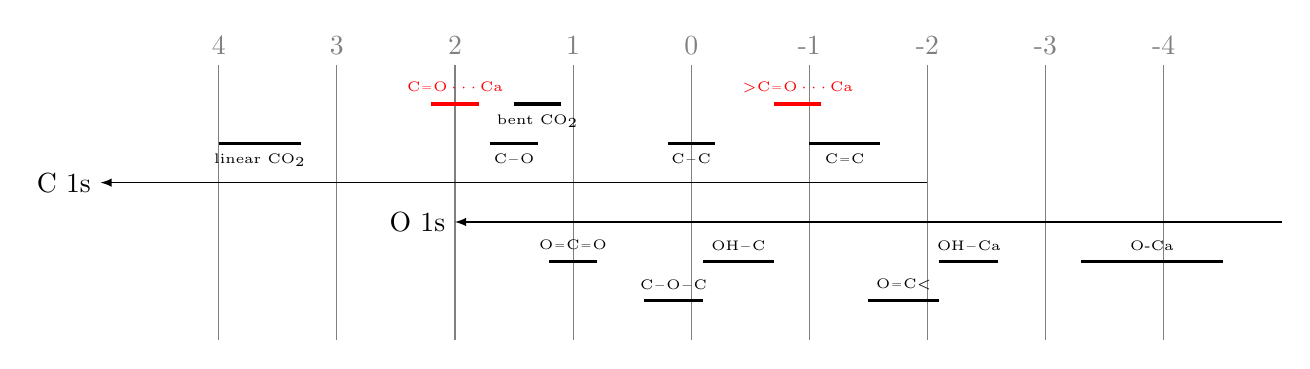
\begin{tikzpicture}[xscale=-1.5]
		\foreach \i in {-4,-3,...,4}{
			\draw[gray] (\i,1.5) node[above]{\i} -- +(0, -3.5);
		}
		%---
		\draw[-latex] (-2,0)  --  (5,0) node[left]{C 1s} ;
		\draw[-latex] (-5,-.5)  --  (2,-.5) node[left]{O 1s} ;
		\draw[very thick] (-.2,.5) -- +(.4,0) node[midway,below]{\tiny\ce{C-C}};
		\draw[very thick] (-1.6,.5) -- +(.6,0) node[midway,below]{\tiny\ce{C=C}};
		\draw[very thick] (3.3,.5) -- +(.7,0) node[midway,below]{\tiny linear \ce{CO2}};
		\draw[very thick] (1.3,.5) -- +(.4,0) node[midway,below]{\tiny\ce{C-O}};
		\draw[very thick] (1.1,1) -- +(.4,0) node[midway,below]{\tiny bent \ce{CO2}};
		\draw[very thick,red] (-1.1,1) -- +(.4,0) node[midway,above]{\tiny$>$\ce{C=O\cdots{}Ca}};
		\draw[very thick,red] (1.8,1) -- +(.4,0) node[midway,above]{\tiny\ce{C=O\cdots{}Ca}};
		%---
		\draw[very thick] (-4.5,-1.) -- +(1.2,0) node[midway,above]{\tiny O-Ca};
		\draw[very thick] (-2.6,-1.) -- +(.5,0) node[midway,above]{\tiny\ce{OH-Ca}};
		\draw[very thick] (.8,-1.) -- +(.4,0) node[midway,above]{\tiny\ce{O=C=O}};
		\draw[very thick] (-2.1,-1.5) -- +(.6,0) node[midway,above]{\tiny\ce{O=C}$<$};
		\draw[very thick] (-.7,-1.) -- +(.6,0) node[midway,above]{\tiny\ce{OH-C}};
		\draw[very thick] (-.1,-1.5) -- +(.5,0) node[midway,above]{\tiny\ce{C-O-C}};
	\end{tikzpicture}
	\caption{Trends among \dbe{} (in \si{\electronvolt}) of C 1s (top) and O 1s (bottom) for compounds \textbf{a}-\textbf{j} when grafted on different surfaces. Red bars indicates change due to interaction with \ce{Ca}.}
	\label{fig:trends}
\end{figure}

\section{Conclusions}\label{sec:conclusions}

In this study, the adsorption of a model system, THF, and of its potential degradation products on various calcium surfaces was investigated using periodic boundary condition DFT calculations. Slabs of calcium (\ce{Ca^0}), its oxide (\ce{CaO}), and its hydride (\ce{CaH2}) were constructed, with full hydroxide coverage also considered for \ce{CaO}. Geometry optimizations were performed for both the bare slabs and the adsorbate-slab complexes. The interactions ranged from van der Waals forces to chemisorption. Two key reaction types were identified: reactions between the adsorbate’s carbon atoms and the surface (notably with \ce{CO2}), and proton transfers between the alcohol moiety in the adsorbate and the \ce{CaO} surface. The first reaction is known to lead to the formation of calcite\cite{dahleSituPreparationCalcium2012}, while the second indicates some of the mechanism for the formation of hydroxyls.

Since XPS provides valuable insights  to experimentalists on the chemical environment of atoms and the transformations they undergo during adsorption, the simulation of these spectra was performed. However, careful attention must be paid to the methodologies employed, as direct comparisons between results can be problematic due to potential inconsistencies across different systems. To address these issues, a thorough assessment of the methodological approaches was first conducted. This evaluation indicates that while the \cpx[n]{0} and \cpx[n]{\varepsilon_{Ar,2s}} protocols are highly reliable for gas-phase molecules, the \cpx{E_\infty} protocol more accurately reproduces experimental trends for calcium slabs and their derivatives.

After validating the methodology, it was applied to the various adsorbate-substrate systems. The reactions between the adsorbate and the surface led,  in certain cases, to significant changes in the O 1s and C 1s spectra, while the Ca 2s binding energies appeared less affected. Notably, the interactions between oxygen and Ca were also clearly observable in the spectra. Our results are in agreement with experimental studies on the adsorption of \ce{CO2} on calcium surfaces, and close to the one of \ce{CaCO3}.\cite{voigtsAdsorptionCO2CO2009}

Taken together, these findings establish trends for analyzing XPS spectra in the context of SEI formation. Future studies will now explore the impact of incorporating boron derivatives or other counterions to coordinate \ce{Ca^2+}. For example, fluorinated byproducts should be important if  \ce{BF4-}, an interesting candidate,\cite{bodinBoronBasedFunctionalAdditives2023} is considered as a component of the electrolyte. However, conducting such research requires a detailed mechanistic understanding of the degradation reactions involving these species,\cite{youngPreventingElectrolyteDecomposition2021,yamijalaStabilityCalciumIon2021,baonguyenInvestigatingAbnormalConductivity2022,nguyenSolvationReductionCoupling2023} and we are currently working on these topics.

\clearpage
\section*{Supplementary Material}

The supplementary material includes: \begin{inparaenum}[(i)]
	\item chemical structures of the 68 molecules from the dataset by Pueyo Bellafont \textit{et al.}\cite{pueyobellafontPredictingCoreLevel2017},
	\item the evolution of surface energies as a function of the number of layers,
	\item a survey of experimental binding energies (BE's) for Ca, CaO, and \ce{CaCO3},
	\item the variation of bulk and surface Ca 2s BE's with increasing slab thickness, and
	\item XPS spectra for selected compounds.
\end{inparaenum}

\begin{acknowledgements}
	This work was supported by the Excellence of Science (EOS) programme  ECOBAT (EOS No. 40007515). 
	The calculations were performed on: \begin{inparaenum}[(i)]
	\item the computers of the Consortium des \'{E}quipements de Calcul Intensif (C\'{E}CI, \url{http://www.ceci-hpc.be}) and particularly those of the Technological Platform of High-Performance Computing, for which the author gratefully acknowledge the financial support of the F.R.S-FNRS, of the Walloon Region, and of the University of Namur (Conventions No.  U.G006.15, U.G018.19, U.G011.22, RW1610468, RW/GEQ2016, RW2110213, and RW2210148), and
	\item on Lucia, the Tier-1 supercomputer of the Walloon Region, infrastructure funded by the Walloon Region (grant agreement No. RW1910247).
	\end{inparaenum} 
\end{acknowledgements}

\section*{Authors declaration}

\subsection*{Conflict of interest}

The authors have no conflicts to disclose.

\subsection*{Authors contributions}

\textbf{Pierre Beaujean:} conceptualization, methodology (lead), investigation, data curation, formal analysis,  validation (equal), writing/original draft preparation (lead), writing/review \& editing (equal). \textbf{Benoît Champagne:} funding acquisition, project administration, resources, methodology (supporting), validation (equal), writing/original draft preparation (supporting), writing/review \& editing (equal).

\section*{Data Availability}

The data (structures, raw values, and analysis scripts) that supports the finding of this study are available at \url{https://github.com/pierre-24/publi-ECOBAT-XPS/}.
Further data are available on request from the corresponding author.


%\clearpage
\bibliography{biblio}
	
\end{document}